\documentclass[a4paper,11pt,oneside]{article}
\usepackage{tgheros}
\usepackage{graphicx,color}
\usepackage{amssymb, amsmath, array}
\usepackage{cover}
\usepackage{comment}

\usepackage[hidelinks]{hyperref}
\usepackage[capitalise,noabbrev]{cleveref}
\usepackage{amsthm}

\numberwithin{equation}{section}

\crefname{equation}{Eq.}{Eqs.}
\Crefname{equation}{Eq.}{Eqs.}

\newtheorem{theorem}{Theorem}

% --- Project metadata ---
\title{When Laplacian-Pyramid Decoding Equals Linearized Instant-NGP Interpolation}
\author{Abel Théo}
\department{School of Computer and Communication Sciences}
\project{Report}
\date{\today}

% Supervisors (name, affiliation)
\responsible{Prof. Jakob Wenzel}{EPFL / RGL}
\supervisor{Zhang Ziyi}{EPFL / RGL}

\begin{document}
\maketitle

\begin{abstract}
Under explicit conditions, the reconstruction obtained from a Laplacian pyramid with a separable tent is pointwise equivalent under the stated conditions, to that of an Instant-NGP–style multiresolution hash grid when per-level outputs are combined through a linear decoder and hashing is collision-free. In this linear regime, both synthesize signals as sums of shifted and dilated tensor-hat basis functions on a dyadic lattice. This highlights a structural bridge between classical multiresolution analysis and modern neural encodings.
\end{abstract}

\section{Introduction}

The Laplacian pyramid reconstructs images by iteratively expanding each level with a separable kernel. In the standard formulation, the \textsc{expand} operator upsamples and filters the coarser level using the Burt--Adelson generating kernel. Decoding proceeds by expand-then-sum across levels \cite{burt1983laplacian}. At the parameter value $a=0.5$, this operator becomes exactly a separable linear (triangular/tent) interpolation. 

Instant-NGP, by contrast, computes at each level a d-linear interpolation of trainable per-vertex features on a grid. The per-level results are typically concatenated and processed by a small MLP \cite{mueller2022instant}. Here, we replace the MLP by a linear sum across levels to isolate the purely linear synthesis. 

Under dyadic scaling, aligned grids, and collision-free hashing (dense grid), the reconstruction produced by both methods is equivalent pointwise. This observation concerns the synthesis (decoding) operator only: when the \textsc{expand} operator uses $a=0.5$, the effective interpolation weights coincide with the separable d-linear tent basis used in Instant-NGP. 


\section{Assumptions}
\label{assumptions}

\begin{itemize}
\item \textbf{Domain and boundaries.}

Periodic domain \(\Omega=[0,1)^d\).
All sums are taken with wrap. With zero padding, the equalities hold pointwise only on the interior.

\item \textbf{Dyadic lattice.}

In Instant-NGP~\cite{mueller2022instant}, the grid resolutions across
levels follow a geometric progression
\[
N_\ell = \big\lfloor N_{\min}\, b^\ell \big\rfloor,
\]
with a typical growth factor $b \in [1.26, 2]$.
This choice ensures overlapping coverage and gradual refinement rather
than exact dyadic doubling.
In this work, we specialize to the dyadic case $b=2$ and assume
phase-aligned grids across levels.
Under these conditions, each level’s lattice coincides with that of a
classical multiresolution analysis, which allows a direct pointwise
equivalence with the Laplacian pyramid synthesis operator.

\item \textbf{Interpolation kernel.}

Separable tent basis:
\begin{equation}
\label{eq:phi}
\Phi(u)=\prod_{i=1}^d \max(1-|u_i|,0).
\end{equation}

Instant-NGP uses \(d\)-linear interpolation at each level, which coincides with \(\Phi\) in \cref{eq:phi} when written in basis form \cite{mueller2022instant}. For the Laplacian pyramid, setting the Burt--Adelson parameter to \(a=0.5\) makes the \textsc{expand} operator equivalent to tent interpolation (triangular weighting) \cite{burt1983laplacian}.


    
Burt and Adelson's generating kernel in one dimension is parameterized by a coefficient $a$ as
\[
\hat w(0)=a,\quad
\hat w(\pm1)=\tfrac14,\quad
\hat w(\pm2)=\tfrac14-\tfrac a2,
\]
under the equal-contribution constraint described in~\cite{burt1983laplacian}.
At $a=\tfrac12$ this yields weights
\[
\hat w = [\,0,\tfrac14,\tfrac12,\tfrac14,0\,],
\]
whose corresponding \textsc{expand} operator (upsample + filter) implements
linear B-spline interpolation.
In the continuous basis view, this reconstruction kernel is exactly
the tent (degree-1 B-spline) function
\[
h(u) = \max(1 - |u|, 0),
\]
applied separably across dimensions:
\[
\Phi(u)=\prod_{i=1}^d h(u_i).
\]
Hence, when the Laplacian pyramid uses $a{=}\tfrac12$, its
\textsc{expand} operator is equivalent to the separable tent
interpolant also used in the linear Instant-NGP grid.

\item \textbf{Aligned grids.}

All levels lie on the same dyadic lattice. There are no per-level shifts.

\item \textbf{Hashing (collision-free).}

At level \(\ell\), injectivity of the corner-index map holds. Under the periodic wrap, we require \(N_\ell^d \le T\) (unique vertices \(=N_\ell^d\)). With open boundaries use \((N_\ell+1)^d \le T\).
In this regime, each level behaves as a dense grid.

\item \textbf{Linear reduction across levels.}
We replace the MLP by a linear sum across levels so the overall decoder is linear.
\end{itemize}

\section{Equivalence of the synthesis operators}

\paragraph{Notation and coordinates.}
We work on the unit cube $\Omega=[0,1)^d$ with dyadic levels
$N_\ell=2^\ell$. Grid nodes are indexed by
$k\in\mathbb{Z}^d$, and continuous coordinates
$x\in\Omega$ are evaluated through the separable tent
basis $\Phi$ of \cref{eq:phi}.

\paragraph{Tent basis expansion.}

For nodal coefficients \(a_\ell[k]\) on the level-\(\ell\) grid, define the continuous expansion (interpolant)
\begin{equation}
\label{eq:expand-ell}
\operatorname{Expand}^{(\ell)}(a_\ell)(x)
=\sum_{k} a_\ell[k]\;\Phi(2^\ell x-k),
\end{equation}
which corresponds to bi/tri/d-linear interpolation expressed in basis form (cf.\ \cref{eq:phi}).

Here, the coefficients \(a_\ell[k]\) represent the discrete values stored at the grid nodes of level~\(\ell\). They correspond to the pixel samples \(g_\ell(i,j)\) in the classical Laplacian pyramid and to the per-corner feature values in the Instant-NGP hash grid.

\paragraph{Hash-grid reconstruction.}
At level~\(\ell\), Instant-NGP computes the d-linear interpolant (Fig.~3 in \cite{mueller2022instant})
\begin{equation}
\label{eq:hash-level}
H_\ell(x)=\sum_k c_\ell[k]\;\Phi(2^\ell x-k).
\end{equation}
In the \emph{linear} variant considered here, the full reconstruction is the sum across levels:
\begin{equation}
\label{eq:hash-sum}
\widehat f_{\mathrm{hash}}(x)
=\sum_{\ell=0}^{L} H_\ell(x)
=\sum_{\ell=0}^{L}\sum_k c_\ell[k]\;\Phi(2^\ell x-k).
\end{equation}
which corresponds to a linear combination across levels.

In the practical Instant-NGP implementation each vertex stores an
$F$-dimensional feature vector $f_\ell[k]$.  A linear per-level readout
$w_\ell\in\mathbb{R}^F$ produces effective scalar coefficients
$c_\ell[k]=w_\ell^\top f_\ell[k]$.
Under this linearization the synthesis in
\cref{eq:hash-level,eq:hash-sum} is identical to that obtained with
scalar nodal values $c_\ell[k]$.


\paragraph{Laplacian-pyramid reconstruction.}
Let \(L_\ell[k]\) denote Laplacian bands for \(\ell=0,\dots,L-1\) and \(G_L[k]\) the coarsest Gaussian residual. Classical reconstruction proceeds by expand-then-sum:
\begin{equation}
\label{eq:lp-recon}
\widehat f_{\mathrm{LP}}(x)
=\sum_{\ell=0}^{L-1}\operatorname{Expand}^{(\ell)}(L_\ell)(x)
+\operatorname{Expand}^{(L)}(G_L)(x),
\end{equation}
i.e.,
\begin{equation}
\label{eq:lp-recon-sum}
\widehat f_{\mathrm{LP}}(x)
=\sum_{\ell=0}^{L-1}\sum_k L_\ell[k]\;\Phi(2^\ell x-k)
+\sum_k G_L[k]\;\Phi(2^L x-k),
\end{equation}
which mirrors the expand-then-sum decoding identity in \cite{burt1983laplacian}.
\paragraph{}
Both formulations can be viewed as expansions in a separable tent basis on a dyadic lattice. The Laplacian pyramid’s coefficients \(\{L_\ell[k], G_L[k]\}\) and the hash grid’s per-level features \(\{c_\ell[k]\}\) therefore play the same structural role as nodal coefficients of the same multiscale basis. The difference lies only in nomenclature: residual bands versus trainable features.

\paragraph{Observation.}
Under the assumptions above, the linear-decoder hash grid and the Laplacian pyramid with tent \textsc{expand} produce identical reconstructions for the coefficient identification
\begin{equation}
\label{eq:coeff-map}
c_\ell[k]=
\begin{cases}
L_\ell[k], & \ell=0,\dots,L-1,\\[2pt]
G_L[k], & \ell=L.
\end{cases}
\end{equation}

\begin{proof}
Substituting \cref{eq:coeff-map} into \cref{eq:hash-sum} and comparing termwise with \cref{eq:lp-recon-sum} gives
\begin{equation}
\begin{aligned}
\widehat f_{\mathrm{hash}}(x)
&=\sum_{\ell=0}^{L}\sum_k c_\ell[k]\;\Phi(2^\ell x-k)\\
&=\sum_{\ell=0}^{L-1}\sum_k L_\ell[k]\;\Phi(2^\ell x-k)
+\sum_k G_L[k]\;\Phi(2^L x-k)\\
&=\widehat f_{\mathrm{LP}}(x)
\end{aligned}
\end{equation}
\end{proof}

\paragraph{Optimization equivalence.}
Because the two reconstructions coincide pointwise under the mapping
\cref{eq:coeff-map}, any differentiable loss $\mathcal{L}(\widehat f)$
induces identical gradients on the per-level coefficients:
\[
\frac{\partial \mathcal{L}}{\partial c_\ell[k]}
= \frac{\partial \mathcal{L}}{\partial L_\ell[k]}.
\]
Consequently, optimizing each level of the Laplacian pyramid proceeds
identically to optimizing the corresponding hash-grid parameters
in the linear regime, which matches our empirical findings in
\cref{fig:losses_all}.

\begin{table}[h]
\centering
\renewcommand{\arraystretch}{1.15} % more vertical breathing room
\setlength{\tabcolsep}{10pt}       % column padding
\caption{Structural correspondence between the Laplacian pyramid and
the linear hash-grid synthesis (under the linear and collision-free assumptions).}
\vspace{0.5em}
\begin{tabular}{
    >{\raggedright\arraybackslash}p{0.27\linewidth}
    >{\centering\arraybackslash}p{0.32\linewidth}
    >{\centering\arraybackslash}p{0.32\linewidth}}
\toprule
\textbf{Concept} & \textbf{Laplacian Pyramid} & \textbf{Linear Hash Grid} \\ 
\midrule
Coefficient symbols & $L_\ell[k],\,G_L[k]$ & $c_\ell[k]$ \\
Interpolation kernel & \textsc{expand}($a{=}0.5$) & d-linear $\Phi$ \\
Grid resolution & $N_\ell = 2^\ell$ & $N_\ell = 2^\ell$ \\
Combination rule & Expand–then–sum & Level-wise sum \\
Domain & Periodic image lattice & Periodic voxel lattice \\
Nonlinear stage & None & Removed MLP \\
\bottomrule
\end{tabular}
\label{tab:structural_correspondence}
\end{table}


\paragraph{}
This equivalence is purely structural: it holds pointwise and linearly under the stated assumptions. Deviations such as non-dyadic scaling, hash collisions, non-tent interpolation, or nonlinear decoders introduce departures from exact equality while preserving the same multiscale tent structure.

\subsection{When the equivalence breaks}
Exact equality holds only under the stated linear, dyadic,
and collision-free assumptions.  Deviations appear when:
\begin{enumerate}
\item $a\neq0.5$: the Burt–Adelson kernel is no longer a tent, so
  the reconstruction kernel differs from the d-linear basis.
\item Hash collisions: non-injective vertex mapping causes
  gradient-averaged coefficients, producing an effective
  low-pass modulation \cite{mueller2022instant}.
\item Nonlinear decoding: an MLP introduces cross-level coupling,
  turning the linear sum into a nonlinear composition.
\item Non-dyadic or shifted grids: mis-aligned phase
  between levels invalidates the pointwise identity.
\item Boundary effects: for open boundaries the equality holds
  only on the interior unless padded.
\end{enumerate}
These deviations are smooth perturbations of the same
multiscale tent expansion.

\section{Experimental verification}

To validate the theoretical equivalence, we optimized a texture
representation under both parameterizations: a Laplacian pyramid with
$a=0.5$ and a linearized Instant-NGP hash grid with collision-free
dense grids.  Both were trained to reproduce the same target image
under an $\ell_2$ loss on pixel intensities.

\paragraph{Implementations.}
For the Laplacian pyramid, we use the publicly available codebase of
Weier et~al.\ \cite{Weier2025PracticalInverse}, configured as a flat
mip-aware image pyramid with tent \textsc{expand} ($a{=}0.5$).
For the hash grid, we use the Mitsuba implementation of the
multiresolution hash-grid encoding with the MLP
removed and a linear level-wise sum as in \cref{eq:hash-sum}.
All experiments are run in Mitsuba using its CUDA
automatic-differentiation backend.

\paragraph{Protocol.}
Each level’s coefficients are optimized independently with identical Adam
hyperparameters and learning-rate schedules.  For the hash grid, we use
three features per level ($F{=}3$) corresponding to the RGB channels of
the Laplacian pyramid, and a linear readout that directly maps them to
color values, yielding effective nodal coefficients $c_\ell[k] \in
\mathbb{R}^3$.  For the Laplacian pyramid, we optimize the per-channel
coefficients $\{L_\ell[k], G_L[k]\}$ directly.  Both parameterizations
are initialized to zero and use identical sampling budgets per
iteration.

\paragraph{Results.}
We first validate the equivalence at the level of the linear synthesis operator, without learning.
Given a target image, we build its Laplacian pyramid \(\{L_\ell, G_L\}\), copy the per-level
coefficients into the corresponding levels of the linear hash grid, and then reconstruct the image
using both decoders under our assumptions. For all tested images
(a \(16\times 16\) checkerboard, a \(1024\times 1024\) checkerboard, the \(512\times 512\)
Lena image, and the \(4096\times 4096\) Claude Lorrain painting
The Embarkation of the Queen of Sheba), the Laplacian-pyramid and hash-grid reconstructions
agree with each other and with the original up to numerical precision. The \(\ell_2\) norm of the
difference between the two reconstructions is exactly zero for the checkerboards and Lena,
and \(1.98\times 10^{-15}\) for the Claude Lorrain image. This residual is on the order of
float-precision rounding error and is therefore consistent with exact equality of the two linear
operators.

\begin{figure}[h]
\centering
\begin{tabular}{ccc}
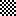
\includegraphics[width=0.3\linewidth]{img/check16x16_original_image.jpg} &
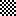
\includegraphics[width=0.3\linewidth]{img/check16x16_pyramid_reconstructed_image.jpg} &
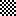
\includegraphics[width=0.3\linewidth]{img/check16x16_hashgrid_neural_texture_image.jpg} \\
\small Original & \small Pyramid Reconstruction & \small Hashgrid Reconstruction \\
\end{tabular}
\caption{Reconstruction comparison for the 16×16 checkerboard pattern.}
\end{figure}

\begin{figure}[h]
\centering
\begin{tabular}{ccc}
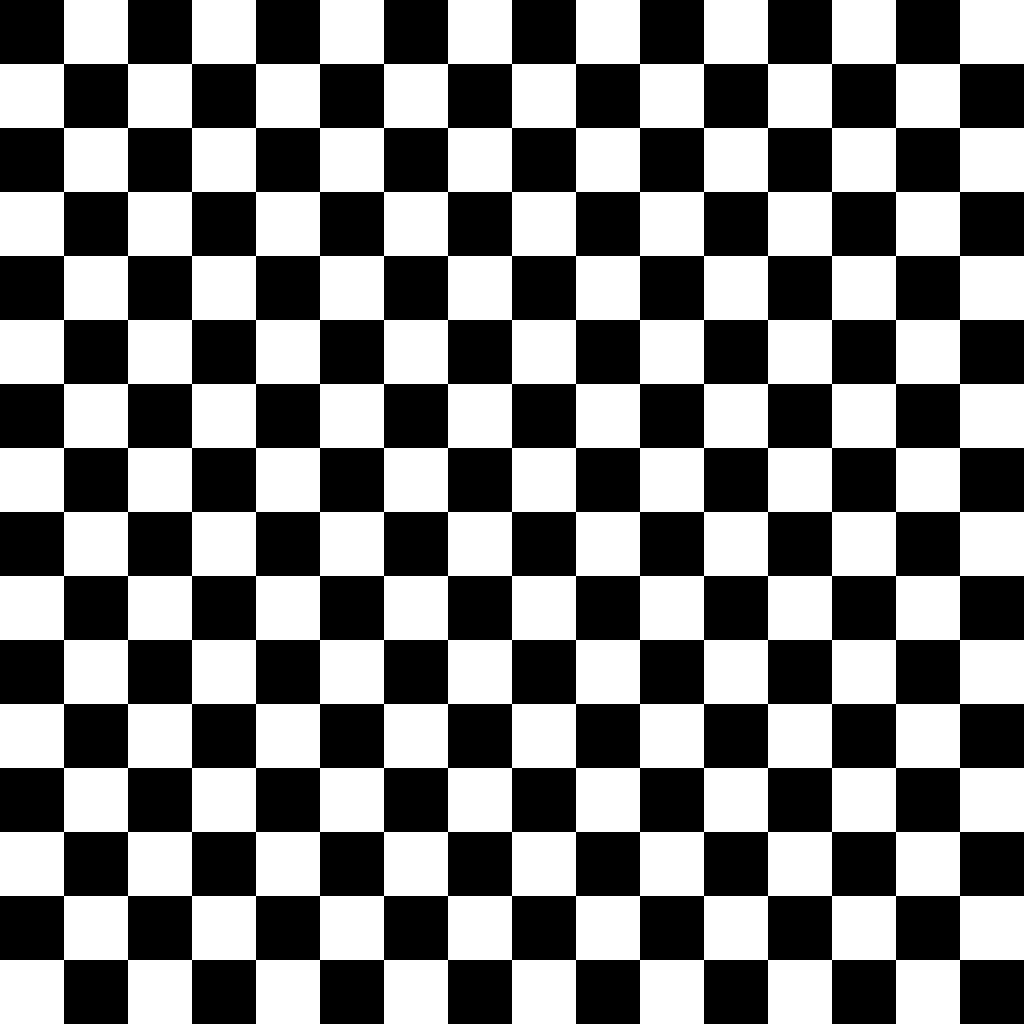
\includegraphics[width=0.3\linewidth]{img/checker_original_image.jpg} &
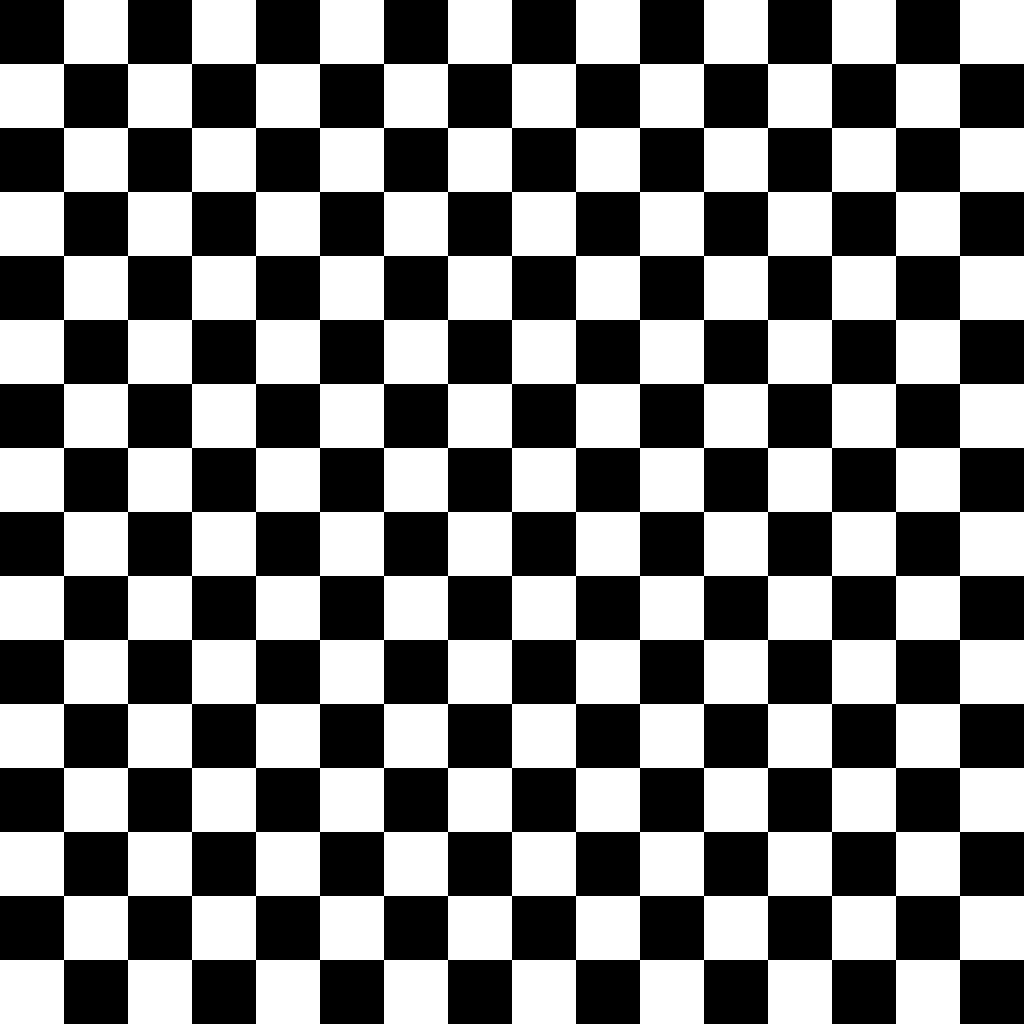
\includegraphics[width=0.3\linewidth]{img/checker_pyramid_reconstructed_image.jpg} &
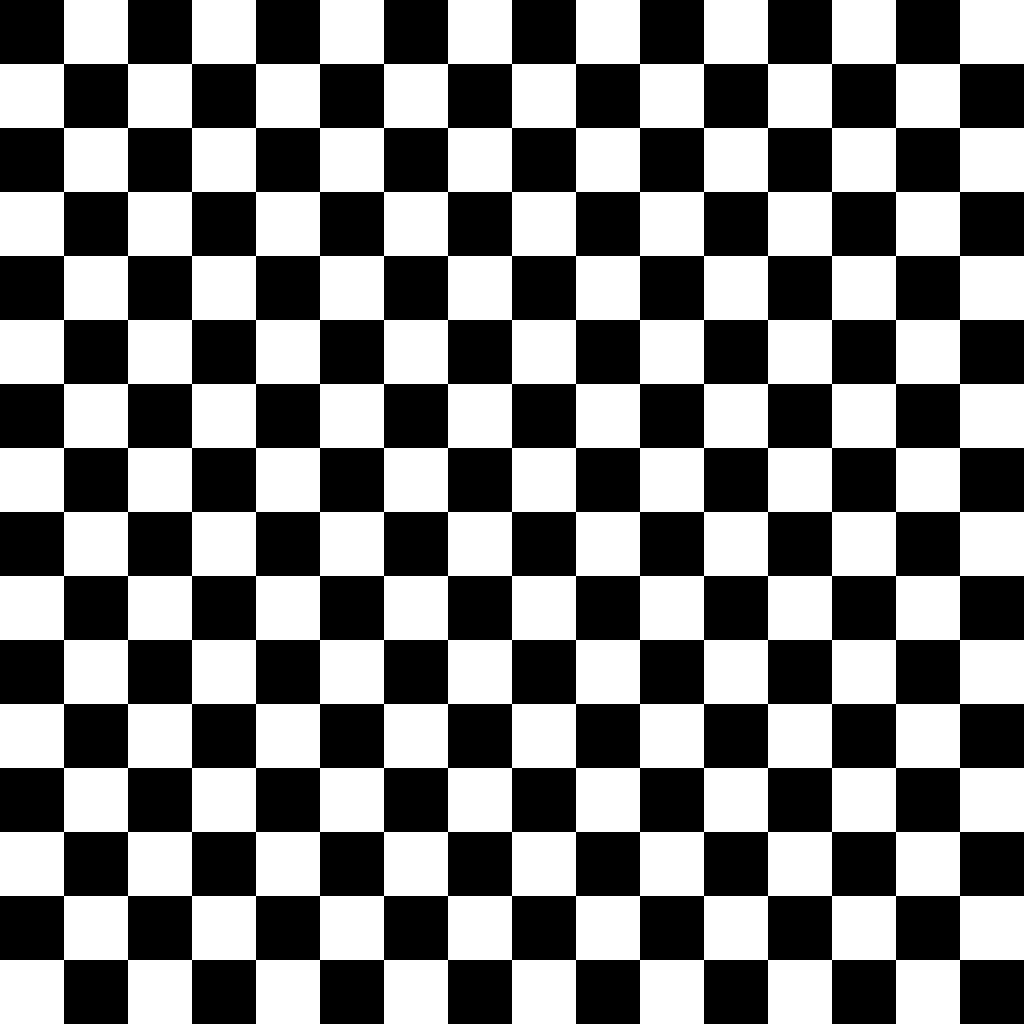
\includegraphics[width=0.3\linewidth]{img/checker_hashgrid_neural_texture_image.jpg} \\
\small Original & \small Pyramid Reconstruction & \small Hashgrid Reconstruction \\
\end{tabular}
\caption{Reconstruction comparison for the 1024×1024 checkerboard pattern.}
\end{figure}

\begin{figure}[h]
\centering
\begin{tabular}{ccc}
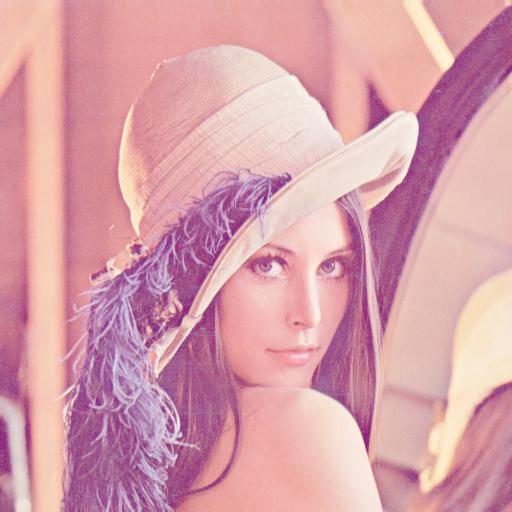
\includegraphics[width=0.3\linewidth]{img/Lenna_original_image.jpg} &
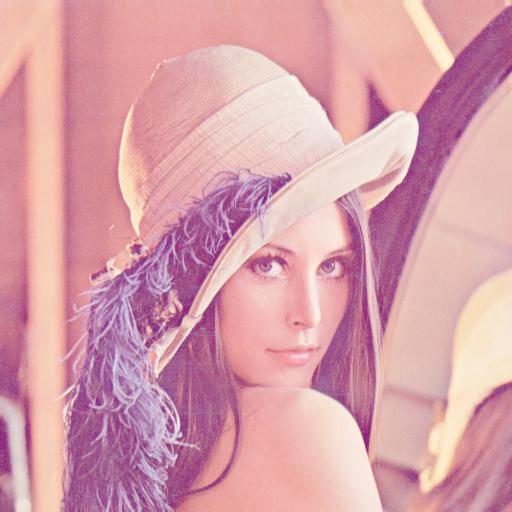
\includegraphics[width=0.3\linewidth]{img/Lenna_pyramid_reconstructed_image.jpg} &
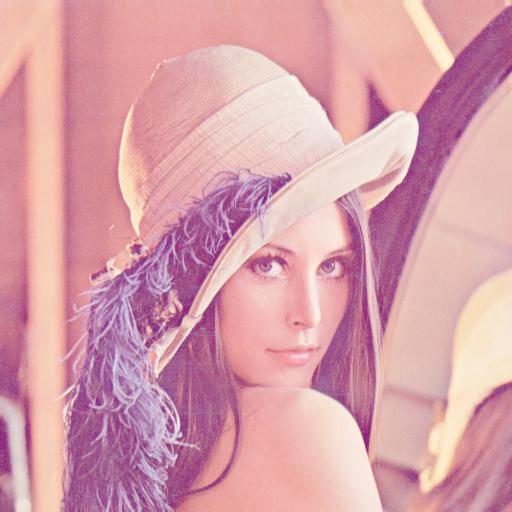
\includegraphics[width=0.3\linewidth]{img/Lenna_hashgrid_neural_texture_image.jpg} \\
\small Original & \small Pyramid Reconstruction & \small Hashgrid Reconstruction \\
\end{tabular}
\caption{Reconstruction comparison for the 512×512 Lena image.}
\end{figure}

\begin{figure}[h]
\centering
\begin{tabular}{ccc}
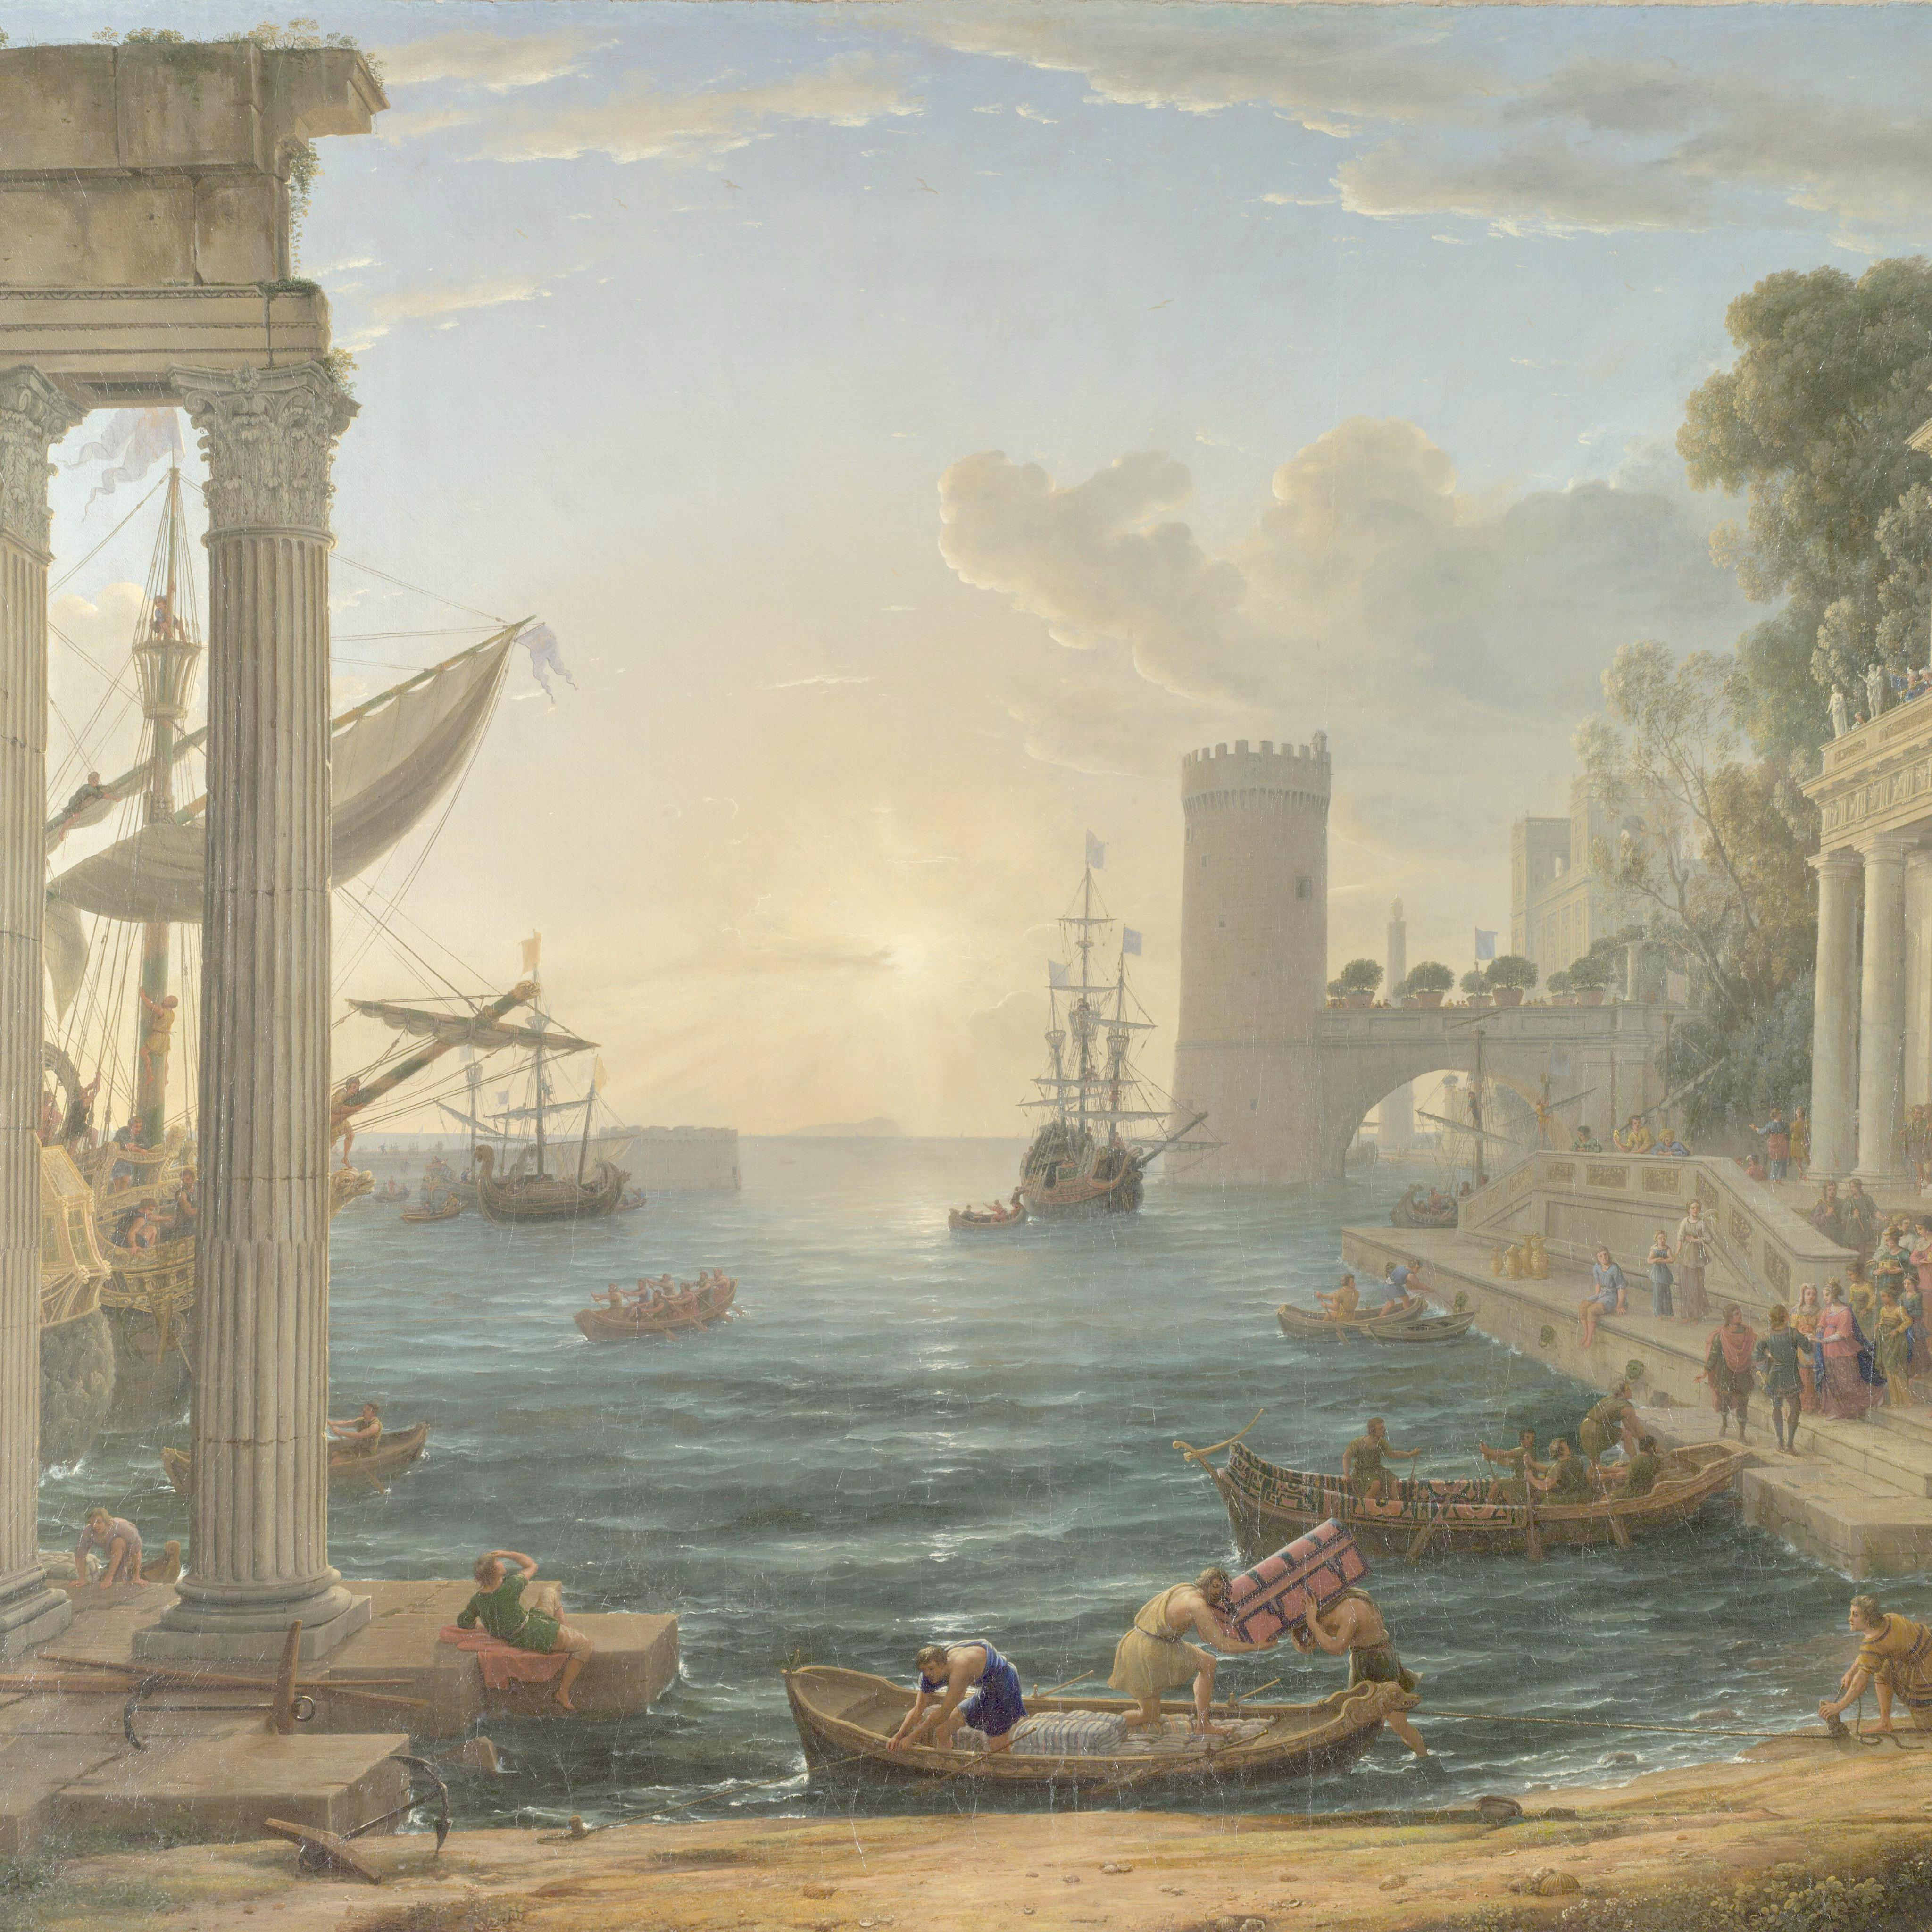
\includegraphics[width=0.3\linewidth]{img/Claude_original_image.jpg} &
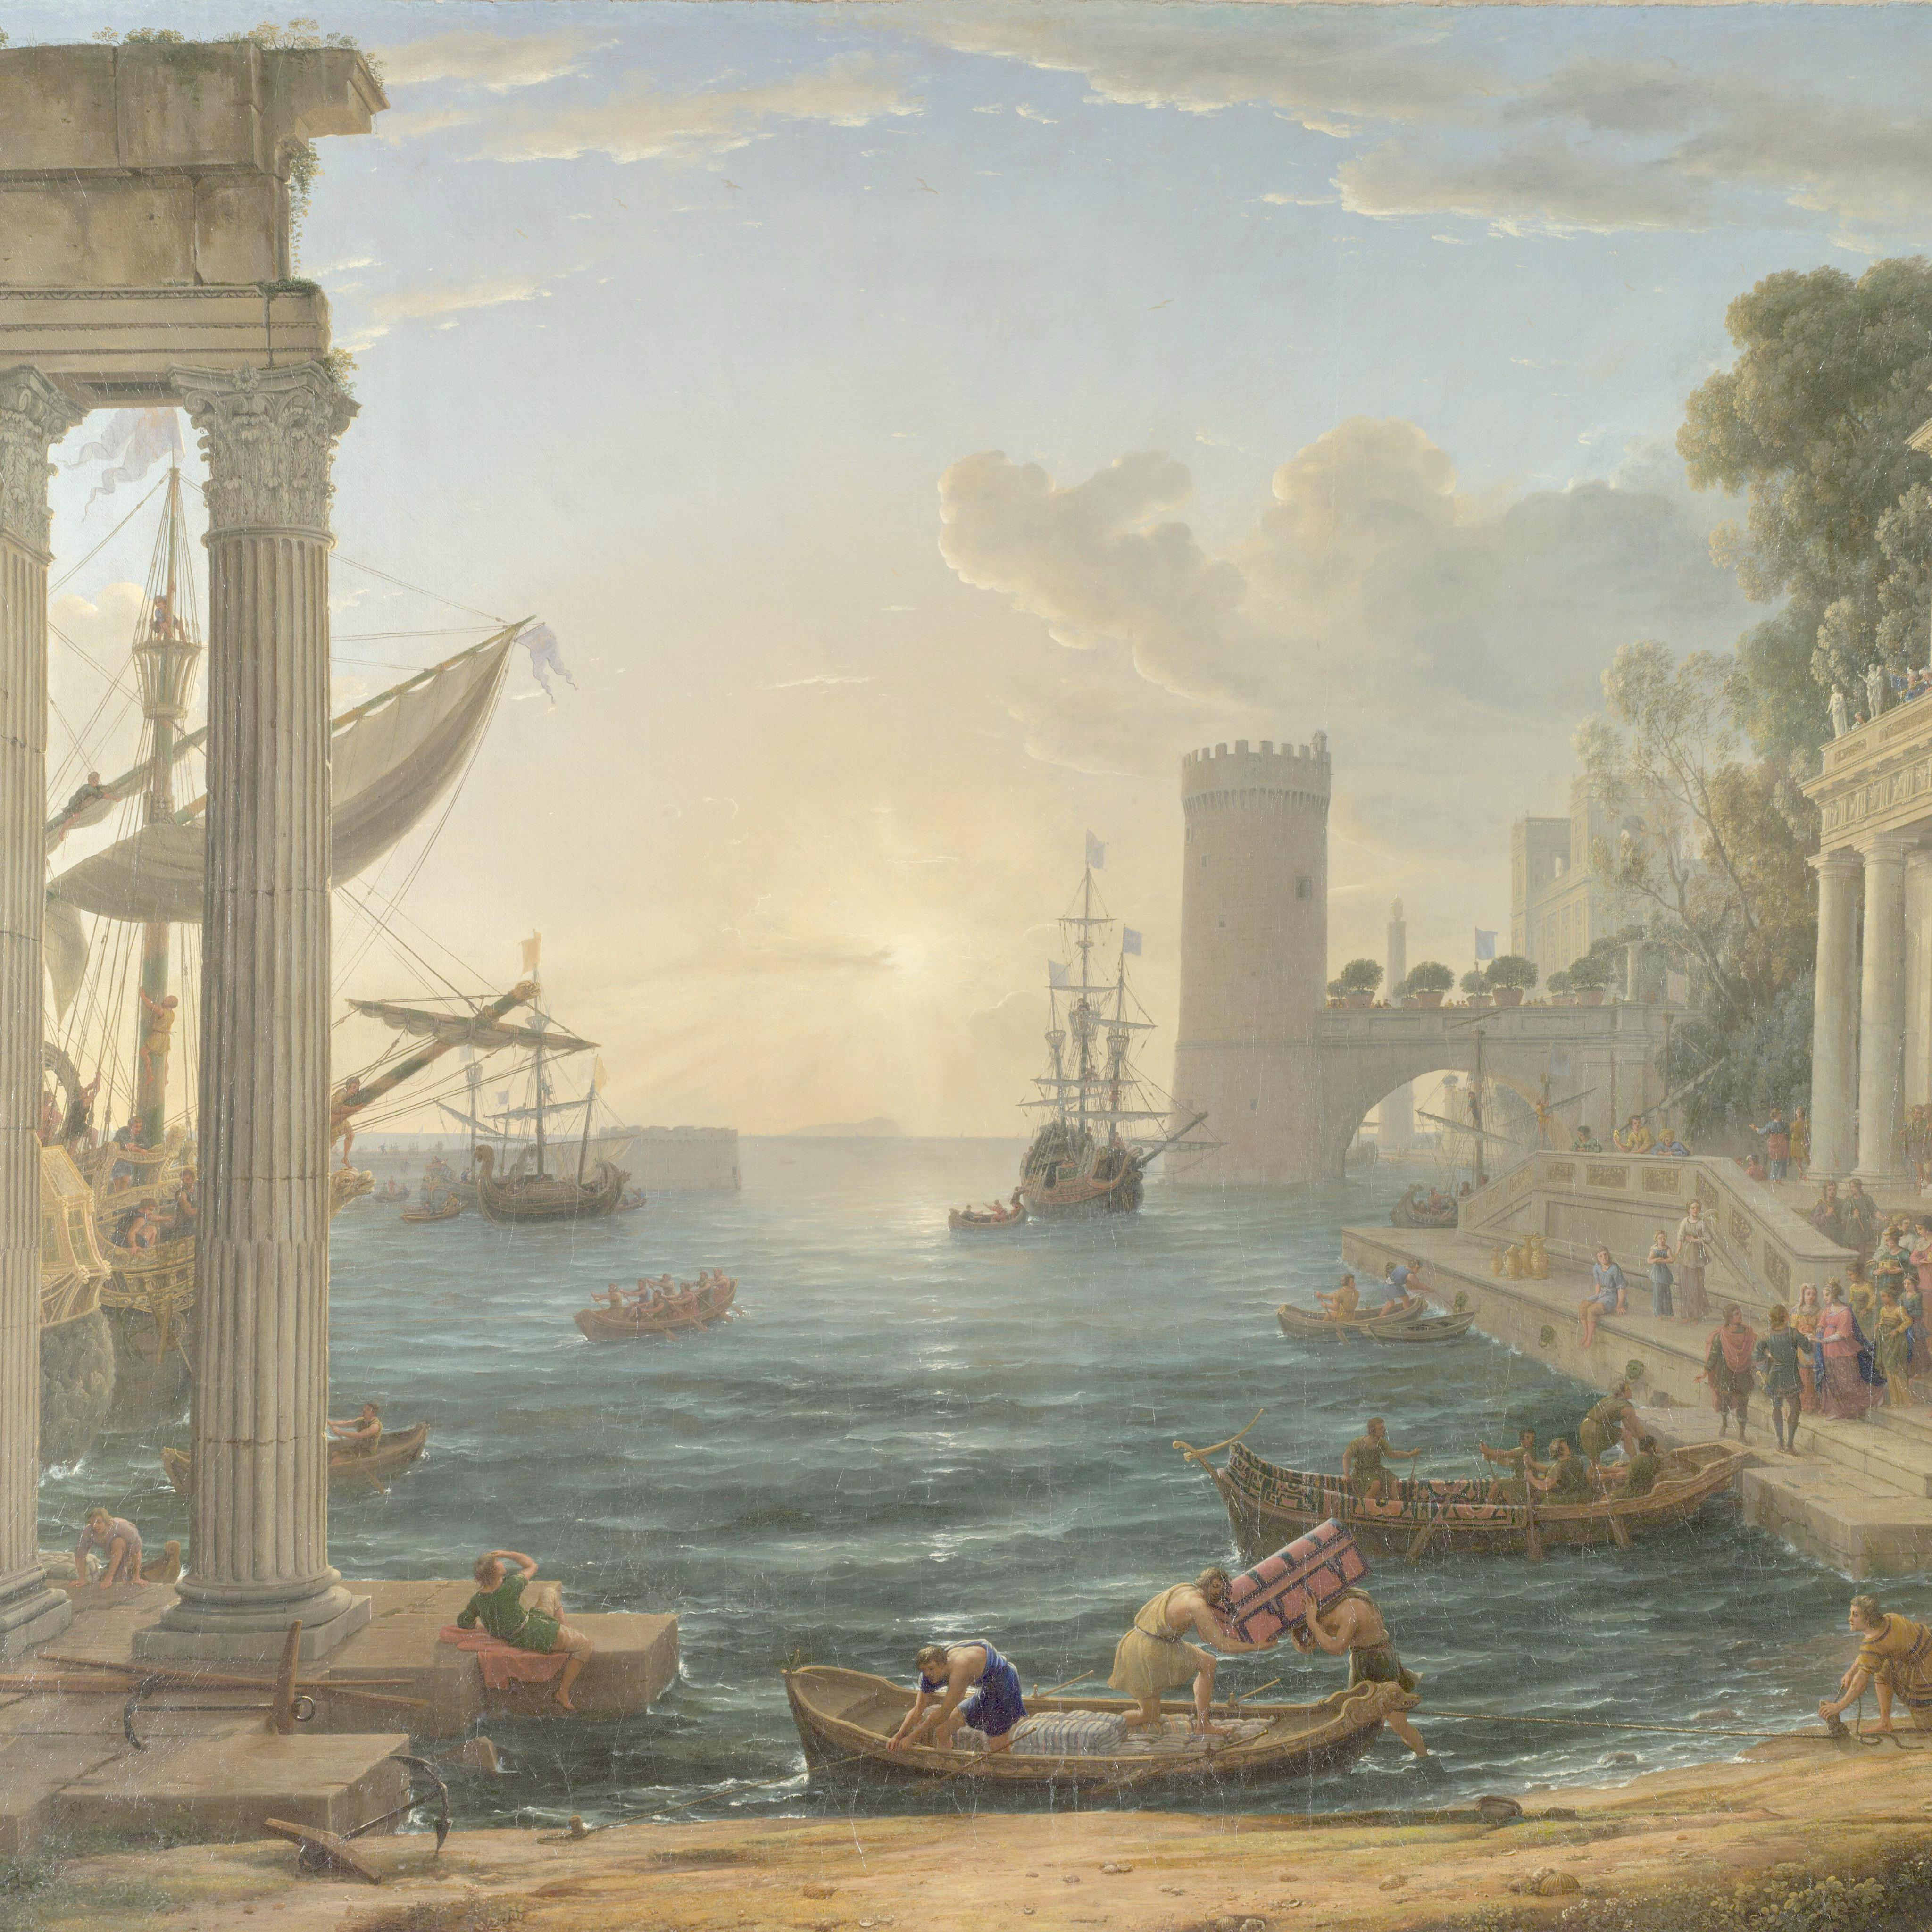
\includegraphics[width=0.3\linewidth]{img/Claude_pyramid_reconstructed_image.jpg} &
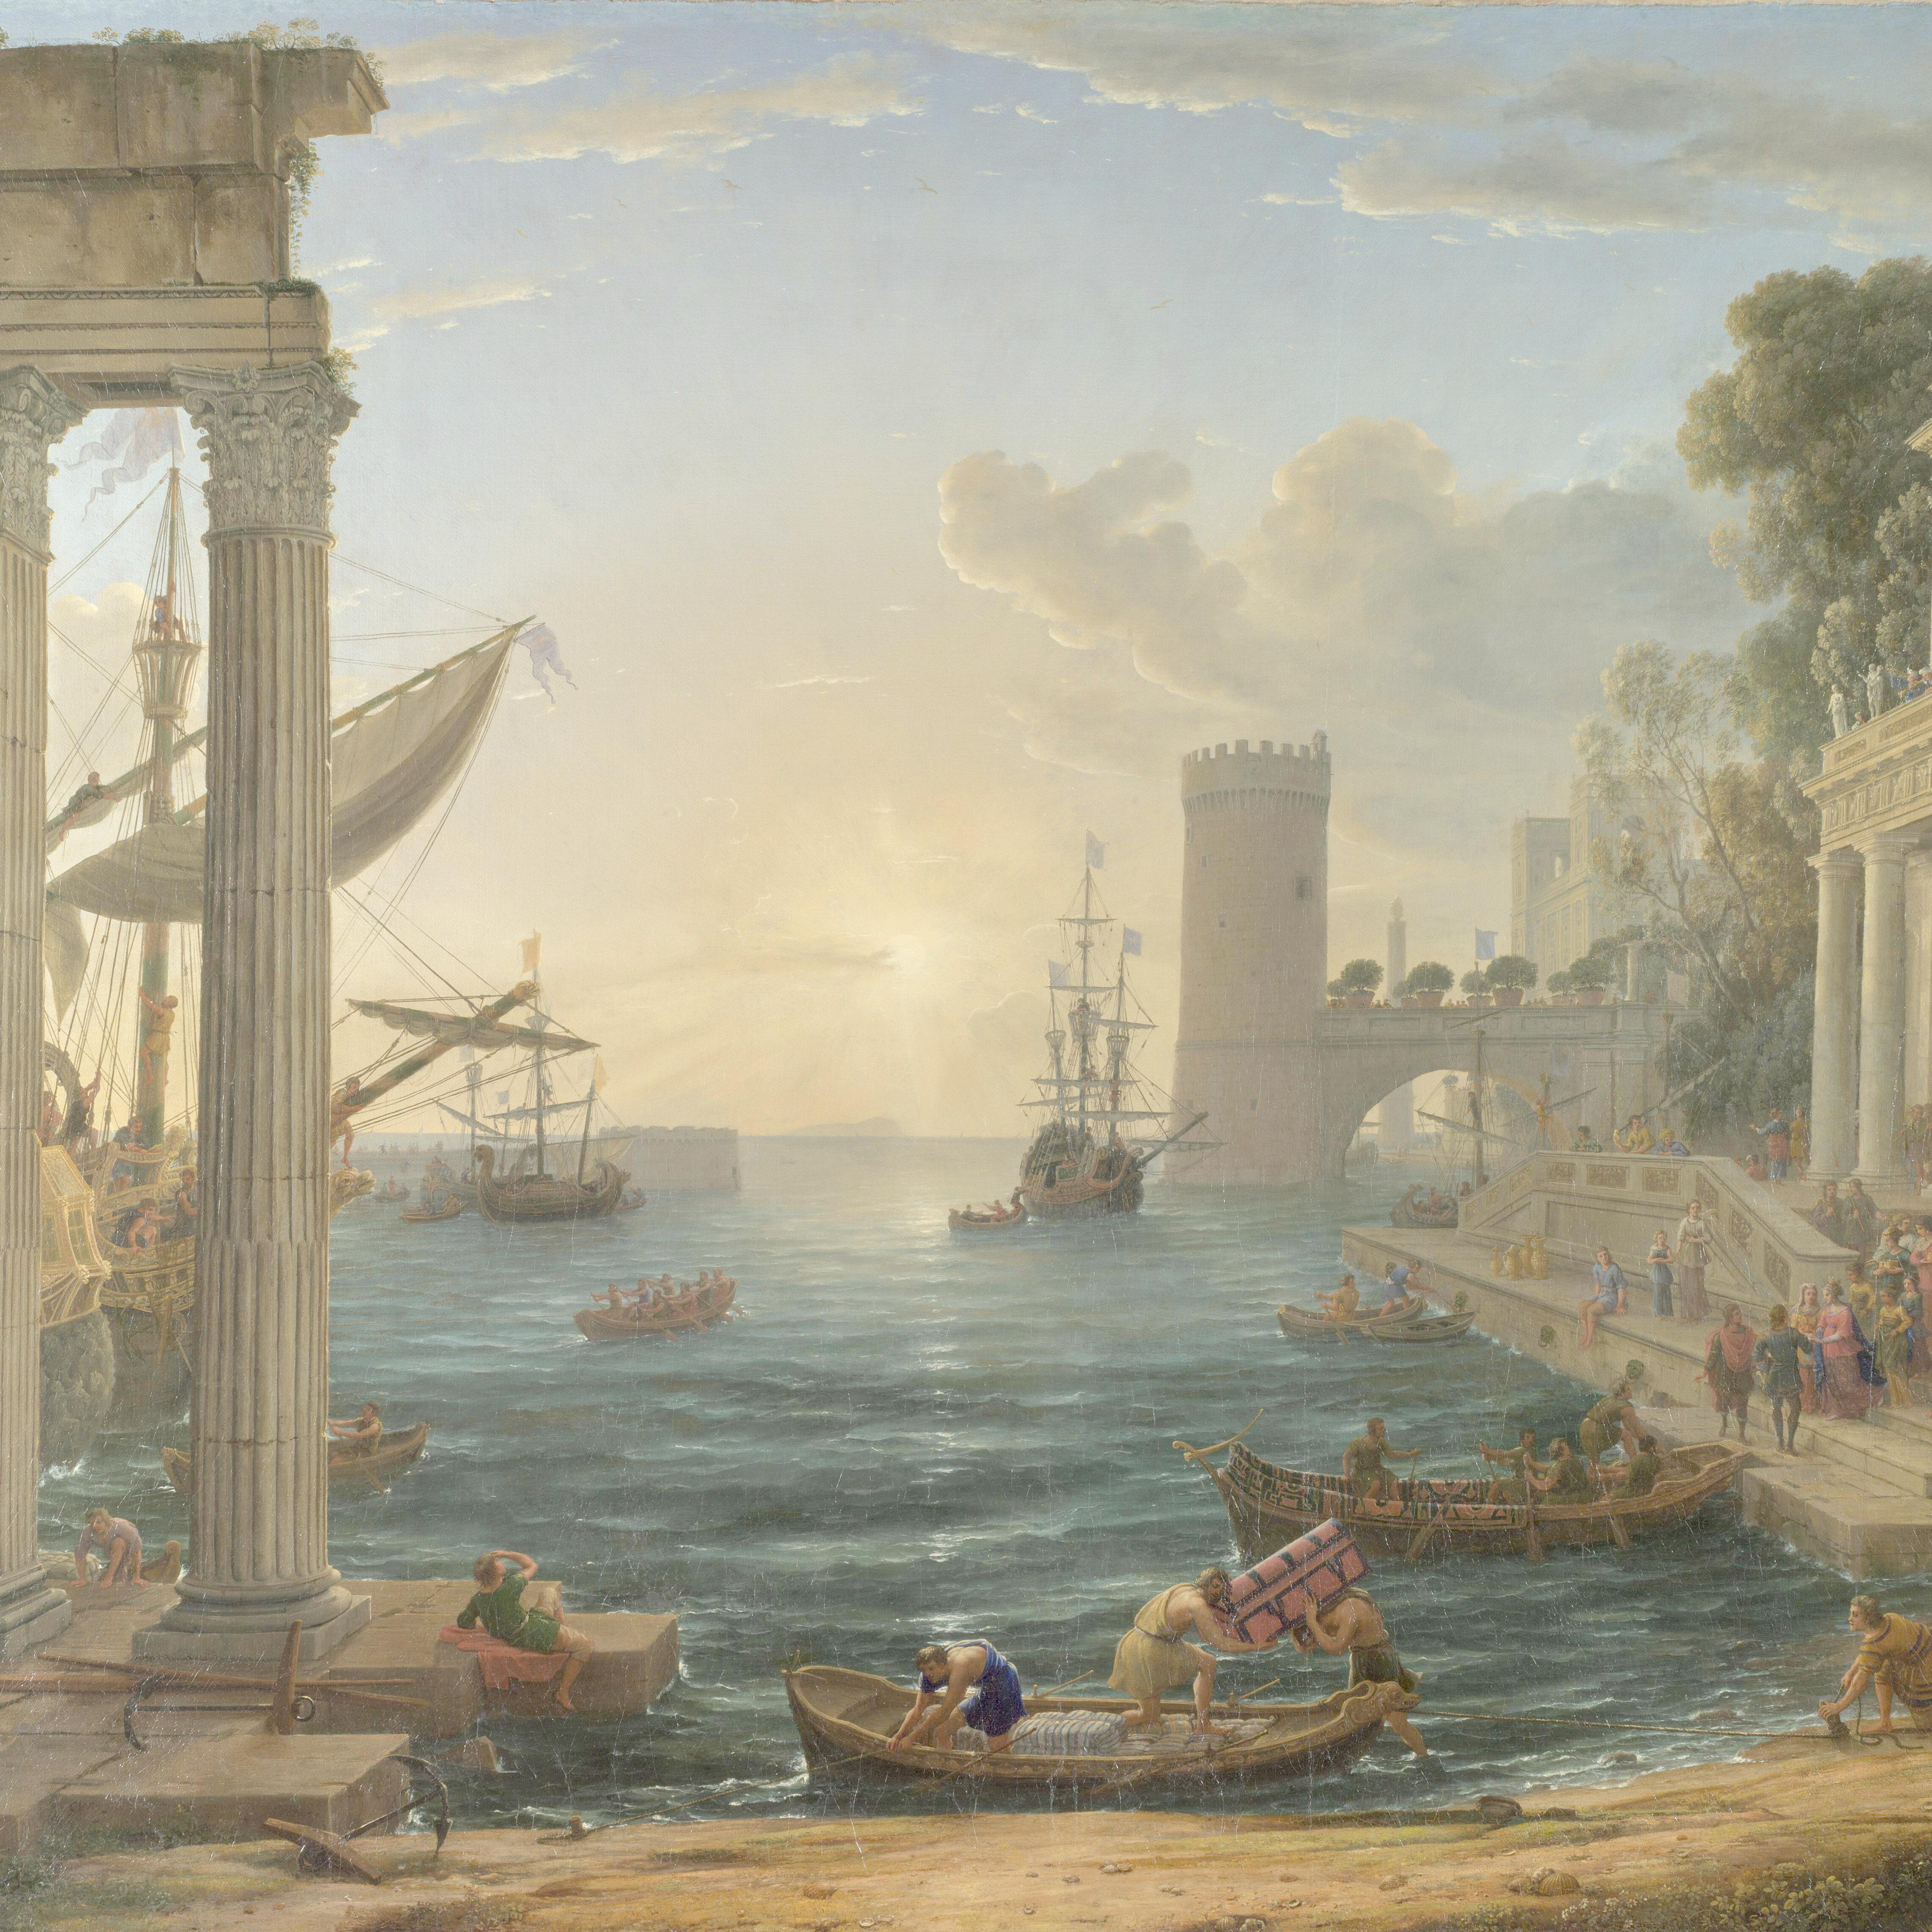
\includegraphics[width=0.3\linewidth]{img/Claude_hashgrid_neural_texture_image.jpg} \\
\small Original & \small Pyramid Reconstruction & \small Hashgrid Reconstruction \\
\end{tabular}
\caption{Reconstruction comparison for the 4096×4096 Claude Lorrain painting.}
\end{figure}


We then place both decoders inside the same optimization loop and fit them independently to several
textures under an \(\ell_2\) reconstruction loss. We consider a \(1024\times 1024\) checkerboard, a \(512\times 512\) Lena, a \(4096\times 4096\) version
of the Claude Lorrain painting, and a \(8192\times 8192\) version of The Great Wave off Kanagawa. For
each case, we train the Laplacian-pyramid and hash-grid parameterizations from the same zero
initialization with identical optimization hyperparameters. The per-iteration loss curves closely
track each other and are visually almost superposed over the full optimization, with only minor
deviations appearing once the loss reaches the \(10^{-5}\) range. The final
reconstructed images are visually indistinguishable. These experiments numerically confirm the analytical equivalence of the two synthesis operators and show that, in the linear regime, the optimization dynamics of the
two parameterizations are effectively the same in practice.

\begin{figure}[h]
\centering
\begin{tabular}{cc}
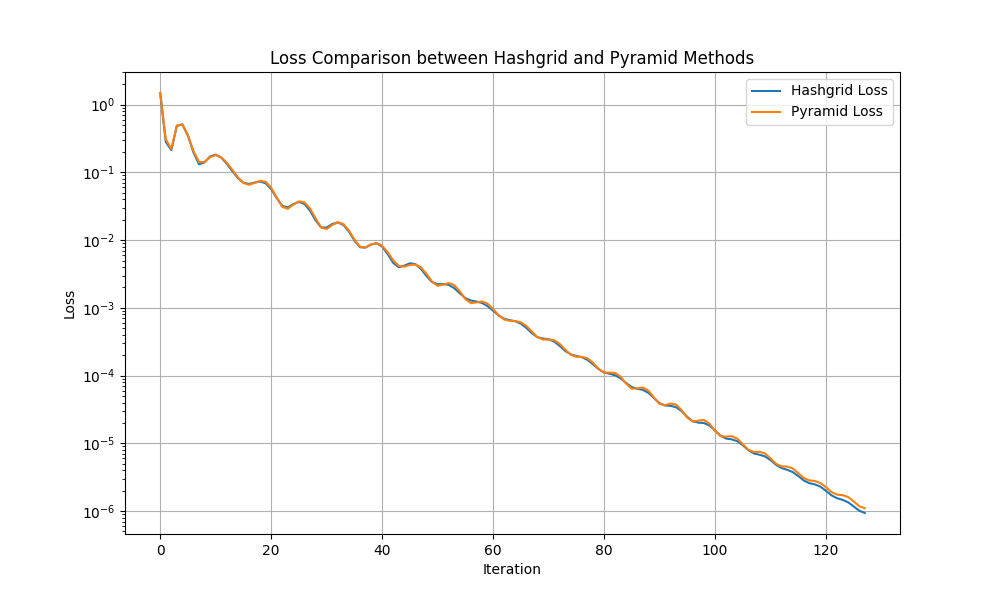
\includegraphics[width=0.45\linewidth]{losses/checker_loss_comparison.png} &
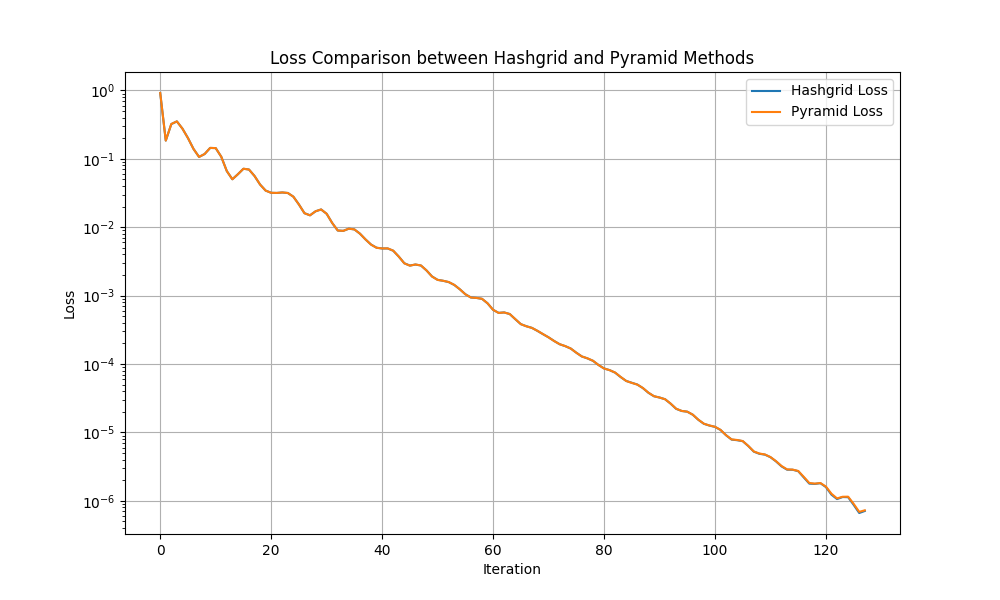
\includegraphics[width=0.45\linewidth]{losses/lenna_loss_comparison.png} \\
\small Checkerboard (1024×1024) & \small Lena (512×512) \\[1em]

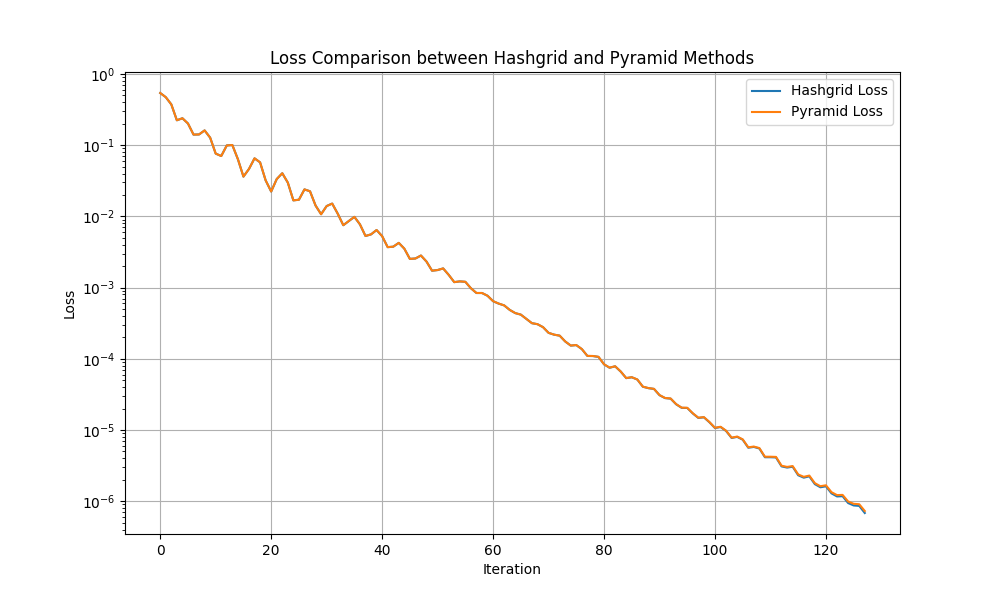
\includegraphics[width=0.45\linewidth]{losses/claude_loss_comparison.png} &
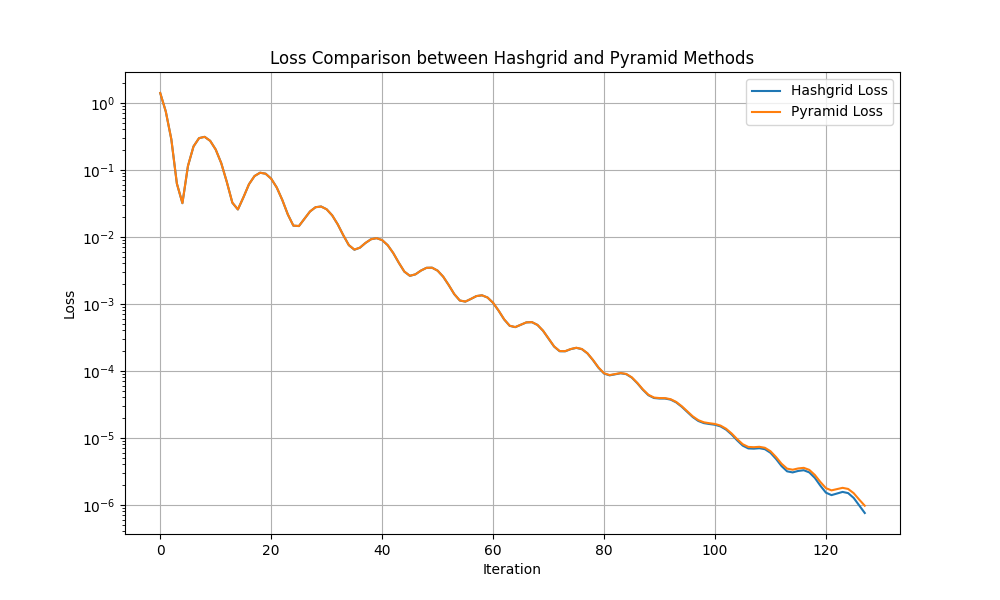
\includegraphics[width=0.45\linewidth]{losses/wave_8k_loss_comparison.png} \\
\small Claude Lorrain (4096×4096) & \small Great Wave (8192×8192)
\end{tabular}
\caption{Loss evolution during texture optimization for four images.
Laplacian-pyramid and linear hash-grid parameterizations exhibit nearly
identical optimization dynamics}
\label{fig:losses_all}
\end{figure}

\newpage



\bibliographystyle{plain}
\bibliography{references}

\end{document}
